\documentclass[10pt,ignorenonframetext,,aspectratio=149]{beamer}
\usefonttheme{serif} % use mainfont rather than sansfont for slide text
\setbeamertemplate{caption}[numbered]
\setbeamertemplate{caption label separator}{: }
\setbeamercolor{caption name}{fg=normal text.fg}
\usepackage{lmodern}
\usepackage{amssymb,amsmath}
\usepackage{ifxetex,ifluatex}
\usepackage{fixltx2e} % provides \textsubscript
\ifnum 0\ifxetex 1\fi\ifluatex 1\fi=0 % if pdftex
  \usepackage[T1]{fontenc}
  \usepackage[utf8]{inputenc}
\else % if luatex or xelatex
  \ifxetex
    \usepackage{mathspec}
  \else
    \usepackage{fontspec}
  \fi
  \defaultfontfeatures{Ligatures=TeX,Scale=MatchLowercase}
  \newcommand{\euro}{€}
    \setmainfont[]{Open Sans}
\fi
% use upquote if available, for straight quotes in verbatim environments
\IfFileExists{upquote.sty}{\usepackage{upquote}}{}
% use microtype if available
\IfFileExists{microtype.sty}{%
\usepackage{microtype}
\UseMicrotypeSet[protrusion]{basicmath} % disable protrusion for tt fonts
}{}
\usepackage{color}
\usepackage{fancyvrb}
\newcommand{\VerbBar}{|}
\newcommand{\VERB}{\Verb[commandchars=\\\{\}]}
\DefineVerbatimEnvironment{Highlighting}{Verbatim}{commandchars=\\\{\}}
% Add ',fontsize=\small' for more characters per line
\usepackage{framed}
\definecolor{shadecolor}{RGB}{248,248,248}
\newenvironment{Shaded}{\begin{snugshade}}{\end{snugshade}}
\newcommand{\AlertTok}[1]{\textcolor[rgb]{0.94,0.16,0.16}{#1}}
\newcommand{\AnnotationTok}[1]{\textcolor[rgb]{0.56,0.35,0.01}{\textbf{\textit{#1}}}}
\newcommand{\AttributeTok}[1]{\textcolor[rgb]{0.77,0.63,0.00}{#1}}
\newcommand{\BaseNTok}[1]{\textcolor[rgb]{0.00,0.00,0.81}{#1}}
\newcommand{\BuiltInTok}[1]{#1}
\newcommand{\CharTok}[1]{\textcolor[rgb]{0.31,0.60,0.02}{#1}}
\newcommand{\CommentTok}[1]{\textcolor[rgb]{0.56,0.35,0.01}{\textit{#1}}}
\newcommand{\CommentVarTok}[1]{\textcolor[rgb]{0.56,0.35,0.01}{\textbf{\textit{#1}}}}
\newcommand{\ConstantTok}[1]{\textcolor[rgb]{0.00,0.00,0.00}{#1}}
\newcommand{\ControlFlowTok}[1]{\textcolor[rgb]{0.13,0.29,0.53}{\textbf{#1}}}
\newcommand{\DataTypeTok}[1]{\textcolor[rgb]{0.13,0.29,0.53}{#1}}
\newcommand{\DecValTok}[1]{\textcolor[rgb]{0.00,0.00,0.81}{#1}}
\newcommand{\DocumentationTok}[1]{\textcolor[rgb]{0.56,0.35,0.01}{\textbf{\textit{#1}}}}
\newcommand{\ErrorTok}[1]{\textcolor[rgb]{0.64,0.00,0.00}{\textbf{#1}}}
\newcommand{\ExtensionTok}[1]{#1}
\newcommand{\FloatTok}[1]{\textcolor[rgb]{0.00,0.00,0.81}{#1}}
\newcommand{\FunctionTok}[1]{\textcolor[rgb]{0.00,0.00,0.00}{#1}}
\newcommand{\ImportTok}[1]{#1}
\newcommand{\InformationTok}[1]{\textcolor[rgb]{0.56,0.35,0.01}{\textbf{\textit{#1}}}}
\newcommand{\KeywordTok}[1]{\textcolor[rgb]{0.13,0.29,0.53}{\textbf{#1}}}
\newcommand{\NormalTok}[1]{#1}
\newcommand{\OperatorTok}[1]{\textcolor[rgb]{0.81,0.36,0.00}{\textbf{#1}}}
\newcommand{\OtherTok}[1]{\textcolor[rgb]{0.56,0.35,0.01}{#1}}
\newcommand{\PreprocessorTok}[1]{\textcolor[rgb]{0.56,0.35,0.01}{\textit{#1}}}
\newcommand{\RegionMarkerTok}[1]{#1}
\newcommand{\SpecialCharTok}[1]{\textcolor[rgb]{0.00,0.00,0.00}{#1}}
\newcommand{\SpecialStringTok}[1]{\textcolor[rgb]{0.31,0.60,0.02}{#1}}
\newcommand{\StringTok}[1]{\textcolor[rgb]{0.31,0.60,0.02}{#1}}
\newcommand{\VariableTok}[1]{\textcolor[rgb]{0.00,0.00,0.00}{#1}}
\newcommand{\VerbatimStringTok}[1]{\textcolor[rgb]{0.31,0.60,0.02}{#1}}
\newcommand{\WarningTok}[1]{\textcolor[rgb]{0.56,0.35,0.01}{\textbf{\textit{#1}}}}
\usepackage{graphicx,grffile}
\makeatletter
\def\maxwidth{\ifdim\Gin@nat@width>\linewidth\linewidth\else\Gin@nat@width\fi}
\def\maxheight{\ifdim\Gin@nat@height>\textheight0.8\textheight\else\Gin@nat@height\fi}
\makeatother
% Scale images if necessary, so that they will not overflow the page
% margins by default, and it is still possible to overwrite the defaults
% using explicit options in \includegraphics[width, height, ...]{}
\setkeys{Gin}{width=\maxwidth,height=\maxheight,keepaspectratio}

% Comment these out if you don't want a slide with just the
% part/section/subsection/subsubsection title:
\AtBeginPart{
  \let\insertpartnumber\relax
  \let\partname\relax
  \frame{\partpage}
}
\AtBeginSection{
  \let\insertsectionnumber\relax
  \let\sectionname\relax
  \frame{\sectionpage}
}
\AtBeginSubsection{
  \let\insertsubsectionnumber\relax
  \let\subsectionname\relax
  \frame{\subsectionpage}
}

\setlength{\emergencystretch}{3em}  % prevent overfull lines
\providecommand{\tightlist}{%
  \setlength{\itemsep}{0pt}\setlength{\parskip}{0pt}}
\setcounter{secnumdepth}{0}

\title{Screen Scraping menggunakan Rvest di R}
\subtitle{(Pelatihan data sains menggunakan R dan Gephi)}
\author{Ujang Fahmi}
\date{}

%% Here's everything I added.
%%--------------------------

\usepackage{graphicx}
\usepackage{rotating}
%\setbeamertemplate{caption}[numbered]
\usepackage{hyperref}
\usepackage{caption}
\usepackage[normalem]{ulem}
%\mode<presentation>
\usepackage{wasysym}
%\usepackage{amsmath}


% Get rid of navigation symbols.
%-------------------------------
\setbeamertemplate{navigation symbols}{}

% Optional institute tags and titlegraphic.
% Do feel free to change the titlegraphic if you don't want it as a Markdown field.
%----------------------------------------------------------------------------------
\institute{Pelajaran ke-6}

% \titlegraphic{\includegraphics[width=0.3\paperwidth]{\string~/Dropbox/teaching/clemson-academic.png}} % <-- if you want to know what this looks like without it as a Markdown field. 
% -----------------------------------------------------------------------------------------------------
\titlegraphic{
\includegraphics[width=0.3\paperwidth]{styles/sadasa.png}}

% Some additional title page adjustments.
%----------------------------------------
\setbeamertemplate{title page}[empty]
%\date{}
\setbeamerfont{subtitle}{size=\small}

\setbeamercovered{transparent}

% Some optional colors. Change or add as you see fit.
%---------------------------------------------------
\definecolor{clemsonpurple}{HTML}{522D80}
 \definecolor{clemsonorange}{HTML}{F66733}
\definecolor{uiucblue}{HTML}{003C7D}
\definecolor{uiucorange}{HTML}{F47F24}


% Some optional color adjustments to Beamer. Change as you see fit.
%------------------------------------------------------------------
\setbeamercolor{frametitle}{fg=clemsonpurple,bg=white}
\setbeamercolor{title}{fg=clemsonpurple,bg=white}
\setbeamercolor{local structure}{fg=clemsonpurple}
\setbeamercolor{section in toc}{fg=clemsonpurple,bg=white}
% \setbeamercolor{subsection in toc}{fg=clemsonorange,bg=white}
\setbeamercolor{footline}{fg=clemsonpurple!50, bg=white}
\setbeamercolor{block title}{fg=clemsonorange,bg=white}


\let\Tiny=\tiny


% Sections and subsections should not get their own damn slide.
%--------------------------------------------------------------
\AtBeginPart{}
\AtBeginSection{}
\AtBeginSubsection{}
\AtBeginSubsubsection{}

% Suppress some of Markdown's weird default vertical spacing.
%------------------------------------------------------------
\setlength{\emergencystretch}{0em}  % prevent overfull lines
\setlength{\parskip}{0pt}


% Allow for those simple two-tone footlines I like. 
% Edit the colors as you see fit.
%--------------------------------------------------
\defbeamertemplate*{footline}{my footline}{%
    \ifnum\insertpagenumber=1
    \hbox{%
        \begin{beamercolorbox}[wd=\paperwidth,ht=.8ex,dp=1ex,center]{}%
      % empty environment to raise height
        \end{beamercolorbox}%
    }%
    \vskip0pt%
    \else%
        \Tiny{%
            \hfill%
		\vspace*{1pt}%
            \insertframenumber/\inserttotalframenumber \hspace*{0.1cm}%
            \newline%
            \color{clemsonpurple}{\rule{\paperwidth}{0.4mm}}\newline%
            \color{clemsonorange}{\rule{\paperwidth}{.4mm}}%
        }%
    \fi%
}

% Various cosmetic things, though I must confess I forget what exactly these do and why I included them.
%-------------------------------------------------------------------------------------------------------
\setbeamercolor{structure}{fg=blue}
\setbeamercolor{local structure}{parent=structure}
\setbeamercolor{item projected}{parent=item,use=item,fg=clemsonpurple,bg=white}
\setbeamercolor{enumerate item}{parent=item}

% Adjust some item elements. More cosmetic things.
%-------------------------------------------------
\setbeamertemplate{itemize item}{\color{clemsonpurple}$\bullet$}
\setbeamertemplate{itemize subitem}{\color{clemsonpurple}\scriptsize{$\bullet$}}
\setbeamertemplate{itemize/enumerate body end}{\vspace{.6\baselineskip}} % So I'm less inclined to use \medskip and \bigskip in Markdown.

% Automatically center images
% ---------------------------
% Note: this is for ![](image.png) images
% Use "fig.align = "center" for R chunks

\usepackage{etoolbox}

\AtBeginDocument{%
  \letcs\oig{@orig\string\includegraphics}%
  \renewcommand<>\includegraphics[2][]{%
    \only#3{%
      {\centering\oig[{#1}]{#2}\par}%
    }%
  }%
}

% I think I've moved to xelatex now. Here's some stuff for that.
% --------------------------------------------------------------
% I could customize/generalize this more but the truth is it works for my circumstances.

\ifxetex
\setbeamerfont{title}{family=\fontspec{Titillium Web}}
\setbeamerfont{frametitle}{family=\fontspec{Titillium Web}}
\usepackage[font=small,skip=0pt]{caption}
 \else
 \fi

% Okay, and begin the actual document...

\begin{document}
\frame{\titlepage}

\begin{frame}
Salam kenal dan selamat datang.

Semoga kita semua bisa saling berbagi pengalaman dan pengetahuan. Saya
adalah Ujang Fahmi, Co-founder dan mentor Sadasa Academy.

\vspace{0.1in}

Jika anda berada dan sedang membaca tutorial ini, maka kemungkinan anda
adalah orang yang sedang ingin belajar data sains, atau mungkin
ditugaskan untuk mempelajari R oleh institusi atau organisasi anda. Sama
seperti saya dulu, dimana tanpa latar belakang enginering saya
didiharuskan untuk belajar R, demi menyelesaikan tugas akhir dan
akhirnya jadilah seperti saya sekarang ini.

\vspace{0.1in}

Satu hal yang pasti, ini adalah langkah pertama dari banyak langkah yang
harus dilalui, entah melalui lembaga resmi atau belajar secara mandiri.
Jadi selamat belajar!!!

\vspace{0.1in}

Ujang Fahmi,

Yogyakarta, 2021-09-27

\vspace{0.1in}

\emph{Materi yang disampaikan disimpan dan dokumentasikan}
\href{https://github.com/eppofahmi/belajaR/tree/master/upn-surabaya}{\textbf{disini}}
\end{frame}

\hypertarget{memahami-web-scrapping}{%
\section{Memahami Web Scrapping}\label{memahami-web-scrapping}}

\hypertarget{apa}{%
\subsection{Apa?}\label{apa}}

\begin{frame}{Apa?}
Web Scarping adalah proses mengumpulkan data tertstruk dari sebuah web
yang biasanya dilakukan secara otomatis. Istilah lain yang juga sering
digunakan adalah ekstraksi data web.

\vspace{0.1in}

Walaupun memiliki tujuan yang kurang lebih sama, web scraping memiliki
perbedaan dengan web crawling. Crawling yang juga digunakan oleh
mesin-mesin pencarian umumnya mengindek semua informasi dari sebuah
tautan atau web halaman demi halaman hingga halaman atau baris terakhir.
Sementara Scraping digunakan untuk mengumpulkan data secara spesifik
dari sebuah tautan atau website.
\end{frame}

\hypertarget{bagaimana}{%
\subsection{Bagaimana?}\label{bagaimana}}

\begin{frame}{Bagaimana?}
\begin{enumerate}
\tightlist
\item
  Web scraping biasanya menggunakan alat yang dibuat secara manual untuk
  melakukan tugas mengambil data spesifik dari sebuah website. Alat
  tersebut umumnya disebut scraper.
\item
  Scraper memanfaatkan data locator/selector untuk
  mendapatkan/mengekstrak data dari file HTML.
\item
  Locator biasanya berupa Xpath, CSS Selector, regex, atau gabungan
  ketiganya.
\end{enumerate}
\end{frame}

\hypertarget{rvest-untuk-scraping}{%
\section{\texorpdfstring{\texttt{Rvest} untuk
scraping}{Rvest untuk scraping}}\label{rvest-untuk-scraping}}

\begin{frame}[fragile]{\texttt{Rvest} untuk scraping}
\texttt{Rvest} merupakan package yang bisa digunakan untuk melakukan
scraping di R. Package ini memiliki fungsi-fungsi untuk mengekstrak:

\begin{enumerate}
\tightlist
\item
  Teks;
\item
  Atribut, seperti url;
\item
  Html nodes; dan
\item
  Tabel
\end{enumerate}

dari dalam sebuah file HTML atau website. Selain itu, \texttt{rvest}
juga memiliki fitur lain sepertu memasukan data pada google form dan
lain sebagainya.
\end{frame}

\hypertarget{mengenal-website}{%
\subsection{Mengenal Website}\label{mengenal-website}}

\begin{frame}{Mengenal Website}
Untuk bisa melakukan scraping maka kita harus terlebih dahulu paham
tentang penyusun sebuah Website yang mungkin sudah tiap hari dikonsumsi.
Sebuah WEB umumnya terdiri dari:

\begin{enumerate}
\tightlist
\item
  HTML untuk menyusun data yang akan ditampilkan;
\item
  CSS untuk mempercantik tampilan data dalam sebuah website; dan
\item
  Javascript untuk mengatur interaksi dalam sebuah web.
\end{enumerate}
\end{frame}

\hypertarget{memilih-tag-html}{%
\subsection{Memilih Tag HTML}\label{memilih-tag-html}}

\begin{frame}[fragile]{Memilih Tag HTML}
\begin{columns}[T]
\begin{column}{0.4\textwidth}
Untuk memilih locator kita bisa melakukan inspect element pada sebuah
website atau menggunakan selectorGadget seperti pada gambar berikut.

Pada web tersebut, misalnya kita ingin mendapatkan judul maka locator
yang bisa digunakan berdasarkan \texttt{selectorGadget} adalah
\texttt{.entry-title\ a}
\end{column}

\begin{column}{0.6\textwidth}
\begin{figure}
\centering
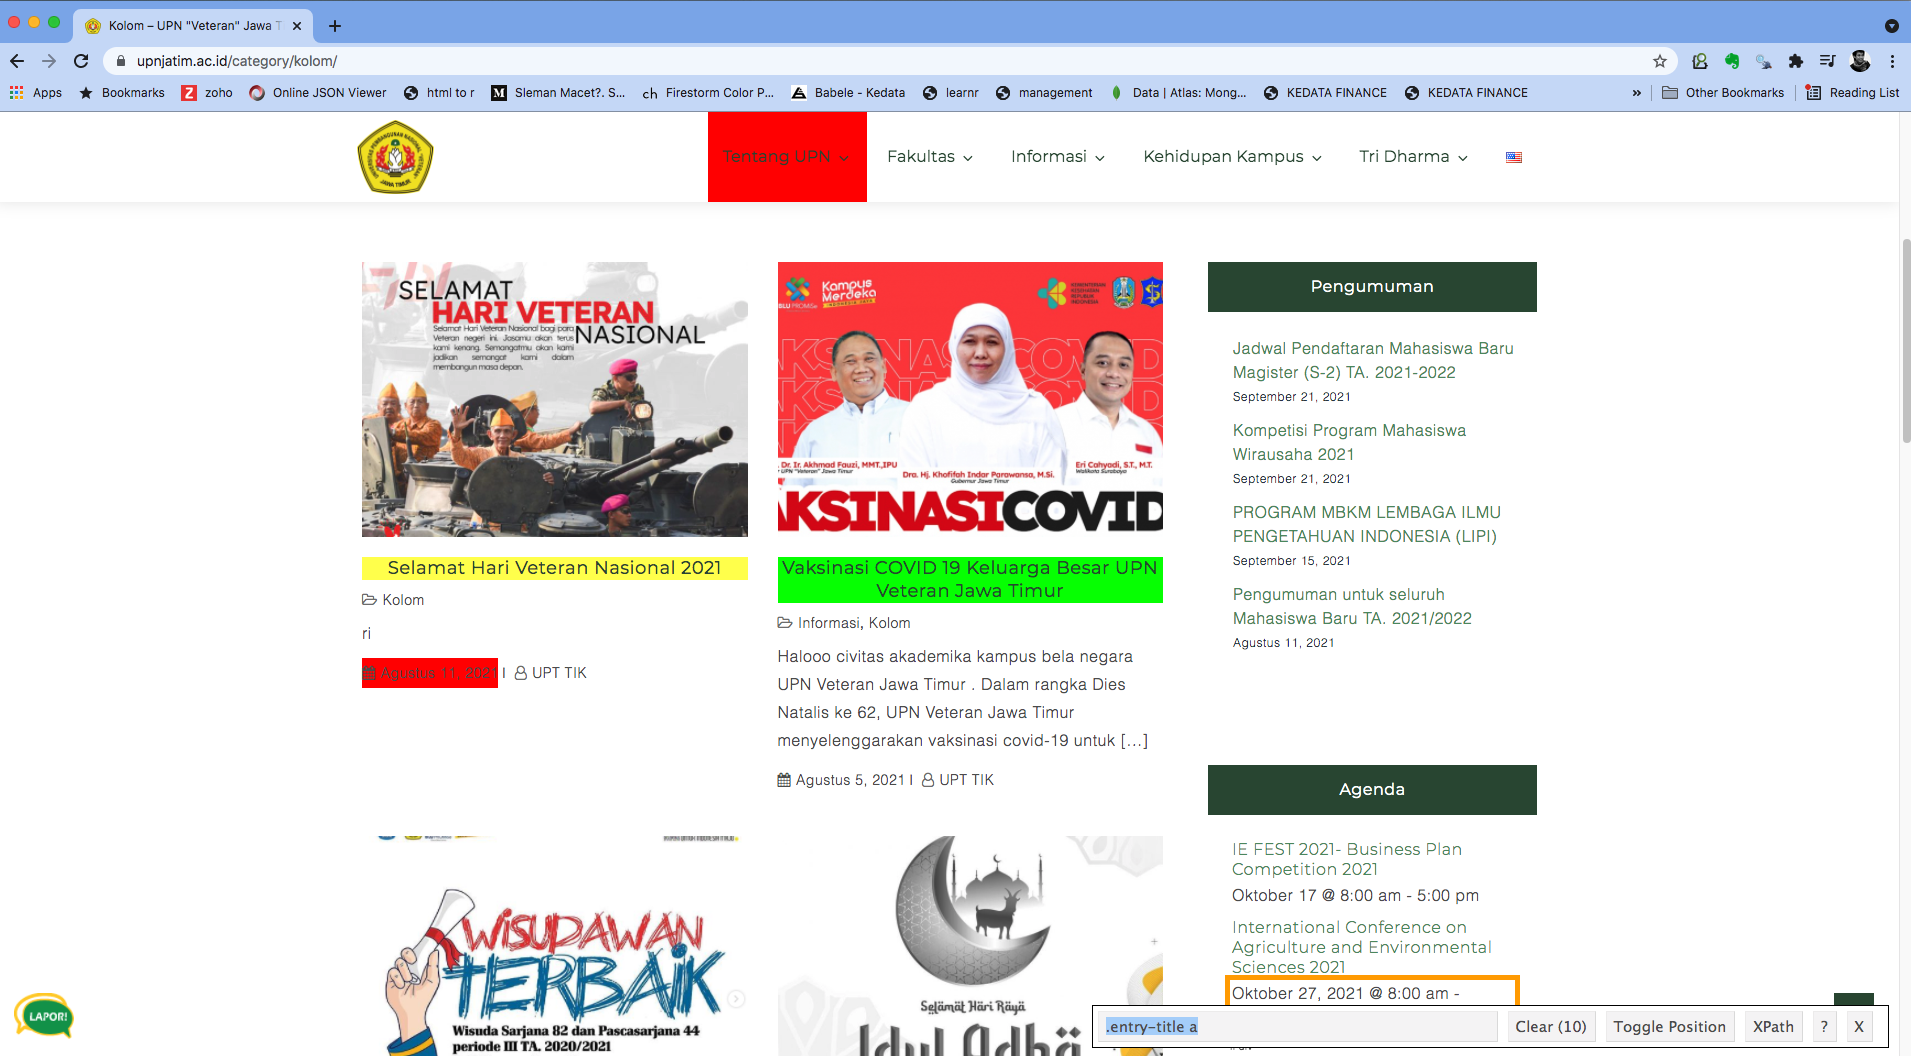
\includegraphics{images/webupn.png}
\caption{Tampilan informasi non akademik UPN Surabaya}
\end{figure}
\end{column}
\end{columns}
\end{frame}

\hypertarget{mengambil-data-dari-tag}{%
\subsection{Mengambil Data dari Tag}\label{mengambil-data-dari-tag}}

\begin{frame}[fragile]{Mengambil Data dari Tag}
Untuk mengambil data dengan cara scraping di R setidaknya kita harus
melakukan dengan tahapan sebagai berikut.

\begin{enumerate}
\tightlist
\item
  Mengunduh html dengan \texttt{read\_html()}
\item
  Menentukan locator/nodes dalam rves dengan \texttt{html\_nodes()}
\item
  Menentukan data yang akan diambil berupa teks, link, atau tabel dengan
  \texttt{html\_text()}, \texttt{html\_attr()} atau
  \texttt{html\_attrs()}, dan \texttt{html\_table()}.
\end{enumerate}
\end{frame}

\hypertarget{persiapan}{%
\section{Persiapan}\label{persiapan}}

\begin{frame}[fragile]{Persiapan}
Untuk bisa melakukan scraping, kita mau tidak mau harus mengenal tag
yang digunakan di HTML. Tag ada penanda umum yang menandai sebuah elemen
dalam html. Untuk itu sebelum melakukan scraping sebaiknya kita tahu.

\begin{enumerate}
\tightlist
\item
  Url web dan kebiasannya
\item
  Konten yang akan diambil
\item
  HTML tag dari konten yang akan diambil (Bisa menggunakan
  \texttt{SelectorGadget})
\end{enumerate}

\texttt{SelectorGadget} merupakan sebuah tool untuk memudahkan memilih
elemen css untuk mendapatkan data yang diingkan. \texttt{SelectorGadget}
bisa didapat dengan menambahkannya pada browser yang anda gunakan. Untuk
chrome bisa klik
\href{https://chrome.google.com/webstore/detail/selectorgadget/mhjhnkcfbdhnjickkkdbjoemdmbfginb?hl=en}{tautan
ini}.
\end{frame}

\hypertarget{url-webpage}{%
\subsection{URL webpage}\label{url-webpage}}

\begin{frame}{URL webpage}
\begin{enumerate}
\item
  Halaman 1:
  \url{https://onlinelibrary.wiley.com/action/doSearch?Ppub=\&field1=AllField\&field2=AllField\&field3=AllField\&text1=public+communication\&text2=pandemic\&text3=\&pageSize=20\&startPage=1}
\item
  Halaman 2:
  \url{https://onlinelibrary.wiley.com/action/doSearch?Ppub=\&field1=AllField\&field2=AllField\&field3=AllField\&text1=public+communication\&text2=pandemic\&text3=\&pageSize=20\&startPage=2}
\item
  Halaman 3:
  \url{https://onlinelibrary.wiley.com/action/doSearch?Ppub=\&field1=AllField\&field2=AllField\&field3=AllField\&text1=public+communication\&text2=pandemic\&text3=\&pageSize=20\&startPage=3}
\end{enumerate}
\end{frame}

\hypertarget{target-data}{%
\subsection{Target data}\label{target-data}}

\begin{frame}{Target data}
Target: Mendapatkan data jurnal dengan katakunci public communication
and pandemic dengan target mendapatkan:

\begin{enumerate}
\tightlist
\item
  Judul
\item
  Penulis
\item
  Tahun; dan
\item
  Link DOI
\end{enumerate}
\end{frame}

\hypertarget{judul}{%
\subsection{Judul}\label{judul}}

\begin{frame}[fragile]{Judul}
urls =
\url{https://onlinelibrary.wiley.com/action/doSearch?field1=AllField\&text1=public+communication\&field2=AllField\&text2=pandemic\&field3=AllField\&text3=\&Ppub=}

\begin{Shaded}
\begin{Highlighting}[]
\FunctionTok{library}\NormalTok{(rvest)}
\NormalTok{url1 }\OtherTok{\textless{}{-}} \FunctionTok{read\_html}\NormalTok{(urls)}

\NormalTok{judul }\OtherTok{\textless{}{-}} \FunctionTok{data\_frame}\NormalTok{(}\AttributeTok{judul =}\NormalTok{ url1 }\SpecialCharTok{\%\textgreater{}\%} 
  \FunctionTok{html\_nodes}\NormalTok{(}\StringTok{\textquotesingle{}.hlFld{-}Title a\textquotesingle{}}\NormalTok{) }\SpecialCharTok{\%\textgreater{}\%} 
  \FunctionTok{html\_text}\NormalTok{(}\AttributeTok{trim =} \ConstantTok{TRUE}\NormalTok{))}
\end{Highlighting}
\end{Shaded}
\end{frame}

\hypertarget{penulis}{%
\subsection{Penulis}\label{penulis}}

\begin{frame}[fragile]{Penulis}
\begin{Shaded}
\begin{Highlighting}[]
\NormalTok{penulis }\OtherTok{\textless{}{-}} \FunctionTok{data\_frame}\NormalTok{(}\AttributeTok{penulis =}\NormalTok{ url1 }\SpecialCharTok{\%\textgreater{}\%} 
  \FunctionTok{html\_nodes}\NormalTok{(}\StringTok{\textquotesingle{}.comma\textquotesingle{}}\NormalTok{) }\SpecialCharTok{\%\textgreater{}\%} 
  \FunctionTok{html\_text}\NormalTok{(}\AttributeTok{trim =} \ConstantTok{FALSE}\NormalTok{))}
\end{Highlighting}
\end{Shaded}
\end{frame}

\hypertarget{tahun}{%
\subsection{Tahun}\label{tahun}}

\begin{frame}[fragile]{Tahun}
\begin{Shaded}
\begin{Highlighting}[]
\NormalTok{tahun\_terbit }\OtherTok{\textless{}{-}} \FunctionTok{data\_frame}\NormalTok{(}\AttributeTok{tahun =}\NormalTok{ url1 }\SpecialCharTok{\%\textgreater{}\%} 
  \FunctionTok{html\_nodes}\NormalTok{(}\StringTok{\textquotesingle{}.meta\_\_epubDate\textquotesingle{}}\NormalTok{) }\SpecialCharTok{\%\textgreater{}\%} 
  \FunctionTok{html\_text}\NormalTok{(}\AttributeTok{trim =} \ConstantTok{FALSE}\NormalTok{))}
\end{Highlighting}
\end{Shaded}
\end{frame}

\hypertarget{doi}{%
\subsection{Doi}\label{doi}}

\begin{frame}[fragile]{Doi}
\begin{Shaded}
\begin{Highlighting}[]
\NormalTok{doi }\OtherTok{\textless{}{-}}\NormalTok{ url1 }\SpecialCharTok{\%\textgreater{}\%}
  \FunctionTok{html\_nodes}\NormalTok{(}\StringTok{".hlFld{-}Title a"}\NormalTok{) }\SpecialCharTok{\%\textgreater{}\%} 
  \FunctionTok{html\_attr}\NormalTok{(}\StringTok{"href"}\NormalTok{)}

\NormalTok{doi }\OtherTok{\textless{}{-}} \FunctionTok{data\_frame}\NormalTok{(doi)}
\NormalTok{doi}\SpecialCharTok{$}\NormalTok{doi }\OtherTok{\textless{}{-}} \FunctionTok{paste0}\NormalTok{(}\StringTok{"https://onlinelibrary.wiley.com"}\NormalTok{, doi}\SpecialCharTok{$}\NormalTok{doi)}

\NormalTok{data\_all }\OtherTok{\textless{}{-}} \FunctionTok{bind\_cols}\NormalTok{(judul, tahun\_terbit, penulis, doi)}
\NormalTok{data\_all}\SpecialCharTok{$}\NormalTok{doi}
\end{Highlighting}
\end{Shaded}
\end{frame}

\hypertarget{your-turn}{%
\section{Your Turn}\label{your-turn}}

\begin{frame}[fragile]{Your Turn}
\begin{quote}
Cobalah lakukan scraping pada sebuah website dengan menggunakan
\texttt{rvest}!
\end{quote}
\end{frame}


\section[]{}
\frame{\small \frametitle{Table of Contents}
\tableofcontents}
\end{document}
